

\documentclass[10pt, a4paper, twocolumn]{article}

\usepackage[english]{babel} % English language hyphenation

\usepackage{microtype} % Better typography

\usepackage{amsmath,amsfonts,amsthm} % Math packages for equations

\usepackage[svgnames]{xcolor} % Enabling colors by their 'svgnames'

\usepackage[hang, small, labelfont=bf, up, textfont=it]{caption} % Custom captions under/above tables and figures

\usepackage{booktabs} % Horizontal rules in tables

\usepackage{lastpage} % Used to determine the number of pages in the document (for "Page X of Total")

\usepackage{graphicx} % Required for adding images

\usepackage{enumitem} % Required for customising lists
\setlist{noitemsep} % Remove spacing between bullet/numbered list elements

\usepackage{sectsty} % Enables custom section titles
\allsectionsfont{\usefont{OT1}{phv}{b}{n}} % Change the font of all section commands (Helvetica)

\usepackage{xcolor}
\usepackage{hyperref}
% https://tex.stackexchange.com/questions/202128/how-to-get-url-and-href-displayed-identically

\hypersetup{colorlinks=true,
linkcolor=black,
urlcolor=gray
% linkcolor=blue,
% urlcolor=blue
}
\urlstyle{rm}

% https://stackoverflow.com/questions/26748820/how-to-change-color-of-hline-in-latex
\usepackage{colortbl}


%----------------------------------------------------------------------------------------
%	MARGINS AND SPACING
%----------------------------------------------------------------------------------------

\usepackage{geometry} % Required for adjusting page dimensions

\geometry{
	top=1cm, % Top margin
	bottom=1.5cm, % Bottom margin
	left=2cm, % Left margin
	right=2cm, % Right margin
	includehead, % Include space for a header
	includefoot, % Include space for a footer
	%showframe, % Uncomment to show how the type block is set on the page
}

\setlength{\columnsep}{7mm} % Column separation width

%----------------------------------------------------------------------------------------
%	FONTS
%----------------------------------------------------------------------------------------

\usepackage[T1]{fontenc} % Output font encoding for international characters
\usepackage[utf8]{inputenc} % Required for inputting international characters

\usepackage{XCharter} % Use the XCharter font

%----------------------------------------------------------------------------------------
%	HEADERS AND FOOTERS
%----------------------------------------------------------------------------------------

\usepackage{fancyhdr} % Needed to define custom headers/footers
\pagestyle{fancy} % Enables the custom headers/footers

\renewcommand{\headrulewidth}{0.0pt} % No header rule
\renewcommand{\footrulewidth}{0.4pt} % Thin footer rule

\renewcommand{\sectionmark}[1]{\markboth{#1}{}} % Removes the section number from the header when \leftmark is used

% \nouppercase\leftmark % Add this to one of the lines below if you want a section title in the header/footer

% Headers
\lhead{} % Left header
\chead{\textit{\thetitle $ $ -- Product Manager}} % Center header - currently printing the article title
\rhead{} % Right header

% Footers
\lfoot{} % Left footer
\cfoot{% % % % %
\href{mailto:venhamon@gmail.com}{venhamon@gmail.com}
|
\href{https://www.linkedin.com/in/bj-pm/}{linkedin.com/in/bj-pm}
|
\href{www.powerinsideout.com}{Coached by powerinsideout.com}
\href{https://www.phyl.org/}{+ NSA}
% Community
| \today
} % Center footer
% \rfoot{\footnotesize
% % Page \thepage\ of \pageref{LastPage}
} % Right footer, "Page 1 of 2"

\fancypagestyle{firstpage}{ % Page style for the first page with the title
	\fancyhf{}
% 	\renewcommand{\footrulewidth}{0pt} % Suppress footer rule
\cfoot{% % % % %
\href{mailto:venhamon@gmail.com}{venhamon@gmail.com}
|
\href{https://www.linkedin.com/in/bj-pm/}{linkedin.com/in/bj-pm}
|
\href{www.powerinsideout.com}{Coached by powerinsideout.com}
\href{https://www.phyl.org/}{+ NSA}
| \today
}
}

%----------------------------------------------------------------------------------------
%	TITLE SECTION
%----------------------------------------------------------------------------------------

\newcommand{\authorstyle}[1]{{\large\usefont{OT1}{phv}{b}{n}\color{DarkRed}#1}} % Authors style (Helvetica)

\newcommand{\institution}[1]{{\footnotesize\usefont{OT1}{phv}{m}{sl}\color{Black}#1}} % Institutions style (Helvetica)

\usepackage{titling} % Allows custom title configuration

\newcommand{\HorRule}{\color{DarkGoldenrod}\rule{\linewidth}{1pt}} % Defines the gold horizontal rule around the title

\pretitle{
	\vspace{-80pt} % Move the entire title section up
	\HorRule\vspace{5pt} % Horizontal rule before the title
	\fontsize{32}{36}\usefont{OT1}{phv}{b}{n}\selectfont % Helvetica
	\color{DarkRed} % Text colour for the title and author(s)
}

\posttitle{\par\vskip 5pt} % Whitespace under the title

\preauthor{} % Anything that will appear before \author is printed

\postauthor{ % Anything that will appear after \author is printed
	\vspace{10pt} % Space before the rule
	\par\HorRule % Horizontal rule after the title
% 	\vspace{0pt} % Space after the title section
}

%----------------------------------------------------------------------------------------
%	ABSTRACT
%----------------------------------------------------------------------------------------

\usepackage{lettrine} % Package to accentuate the first letter of the text (lettrine)
\usepackage{fix-cm}	% Fixes the height of the lettrine

\newcommand{\initial}[1]{ % Defines the command and style for the lettrine
	\lettrine[lines=3,findent=4pt,nindent=0pt]{% Lettrine takes up 3 lines, the text to the right of it is indented 4pt and further indenting of lines 2+ is stopped
		\color{DarkGoldenrod}% Lettrine colour
		{#1}% The letter
	}{}%
}

\usepackage{xstring} % Required for string manipulation

\newcommand{\lettrineabstract}[1]{
	\StrLeft{#1}{1}[\firstletter] % Capture the first letter of the abstract for the lettrine
	\initial{\firstletter}\textbf{\StrGobbleLeft{#1}{1}} % Print the abstract with the first letter as a lettrine and the rest in bold
}

%----------------------------------------------------------------------------------------
%	BIBLIOGRAPHY
%----------------------------------------------------------------------------------------

% \usepackage[backend=bibtex,style=authoryear,natbib=true]{biblatex} % Use the bibtex backend with the authoryear citation style (which resembles APA)
%
% \addbibresource{example.bib} % The filename of the bibliography

% \usepackage[autostyle=true]{csquotes} % Required to generate language-dependent quotes in the bibliography

%%%%%%%%%%%%%%%%%%%%%%%%%%%%%%%%%%%%%%%%%
% Wenneker Article
% Structure Specification File
% Version 1.0 (28/2/17)
%
% This file originates from:
% http://www.LaTeXTemplates.com
%
% Authors:
% Frits Wenneker
% Vel (vel@LaTeXTemplates.com)
%
% License:
% CC BY-NC-SA 3.0 (http://creativecommons.org/licenses/by-nc-sa/3.0/)
%
%%%%%%%%%%%%%%%%%%%%%%%%%%%%%%%%%%%%%%%%%

%----------------------------------------------------------------------------------------
%	PACKAGES AND OTHER DOCUMENT CONFIGURATIONS
%----------------------------------------------------------------------------------------
 % Specifies the document structure and loads requires packages
\showhyphens{syllable breaking algorithm opportunities}


\title{Benji J} % The article title

\author{
	\authorstyle{Product Manager [SaaS,
	Music,
	Crypto---Blockchain---Web3%
	] 	% 	and Mobile App,
	} \\ \\
	\noindent\fbox{%
    \parbox{\textwidth}{%
%         The quick brown fox jumps right over the lazy dog. the quick brown fox jumps right over the lazy dog.
% %
\textbf{This Document Goal}
is to better understand:
1) what I have to offer, how the market sees me;
2) opportunities I haven’t considered; and
3) connect with people you think I should talk with. \\ \\
% %
\textbf{Candidate-Market Fit [CMF]} \\ \textit{%
% 1.
% Seeking a remote \textbf{Product Manager} role with attention to UX at an early stage (Series C, Pre-IPO/ICO) \textbf{Crypto} B2C company with emphasis on social impact, real-life assets, music and media industries.
% 2.
Seeking a remote \textbf{Product Manager} role at an early stage (Series C, or younger) B2C company focused on \textbf{Crypto} in the entertainment or media industry.
\\
\#crypto
\#IP-rights
\#real-world-assets
\#music
\#streaming
\#growth
\#NFTs
\#AI
\#UX
\#B2C
\#B2B2C
% \#B2B
% Seeking a Product Manager remote role with attention to UX at a Series-A to C SaaS-based tech company in Crypto, ideally with social impact, B2C or B2B2C.
% Ideal: based in Argentina or Latin America, in Spanish or Portuguese.
% \\
% Location preference: Remote, NYC timezone. OK travel 3/4 times per year
% \\ \\
}
% \textbf{This Document Goal}
% is to better understand:
% 1) what I have to offer, how the market sees me;
% 2) opportunities I haven’t considered; and
% 3) connect with people you think I should talk with.
    }%
}
\\ \\
%
\textbf{Summary} \\
With a background in Sociology
and Systems Analysis%
,
Benji has been in Product Management %roles
for 5+ years.
% building with design and development teams, as with UXR, QA, Marketing, Support and Operations.
% % % % PM Actions
% Attends to UX flows, copywriting, research, data analytics, strategy and growth.
% https://medium.com/joys-wishful-thinking/top-10-product-management-superpowers-e21c670b3a20
He works in small teams to create impactful launches from ideation to post-launch.
His product super powers include:
rallying a %proper
vision for %biggest
impact,
collaborating and brainstorming to bring out the best from the team,
and completing delivery launches timely with a big picture view.
\\ \\
% % %
% Likes Web3/Crypto, %as a needed personal tool for stable coins,
% and learning about finance and IP rights. \\ \\
\textbf{Career Goals} \\ % % % % % % % % % % % %
% % % % % % % % % % % % Add milestones, Yaron Cohen says
\textit{Short-Term (6 months)} \\
Strengthen Core Skills:
Take product certification/s @scrum.org, attend industry conference.
% Write user stories to gain understanding across teams.
% Tools: Use operational data to measure, build and launch.
\\ \\ % % % % % % % % % % % %
  \textit{Mid-Term (2/3 years)} \\
Expand Impact: offer mentorship, lead a workshop, collaborate with NGOs.
%   Develop strategy skills, focus on user/s journey, discovery, becoming data-metric fluent, positive team impact
\\ \\ % % % % % % % % % % % %
\textit{Long-Term (5/15 years)} \\
Lead:
start own venture, or join an early-stage startup as a co-founder or key team member.
% Clarifying and resolving ambiguity at a high business level.
% Nurture a vision, mission, new market segments %\\ \\
% % % % % % % % % % % %
% \hrule
% }
%
% \noindent\fbox{%
%     \parbox{\textwidth}{%
% \textbf{This Document Goal}
% is to better understand:
% 1) what I have to offer, how the market sees me;
% 2) opportunities I haven’t considered; and
% 3) connect with people you think I should talk with.
% %         The quick brown fox jumps right over the lazy dog. the quick brown fox jumps right over the lazy dog. the quick brown fox jumps right over the lazy dog. the quick brown fox jumps right over the lazy dog. the quick brown fox jumps right over the lazy dog. the quick brown fox jumps right over the lazy dog. the quick brown fox jumps right over the lazy dog. the quick brown fox jumps right over the lazy dog.
%     }%
% }
}

\date{ }

%----------------------------------------------------------------------------------------

\begin{document}
% 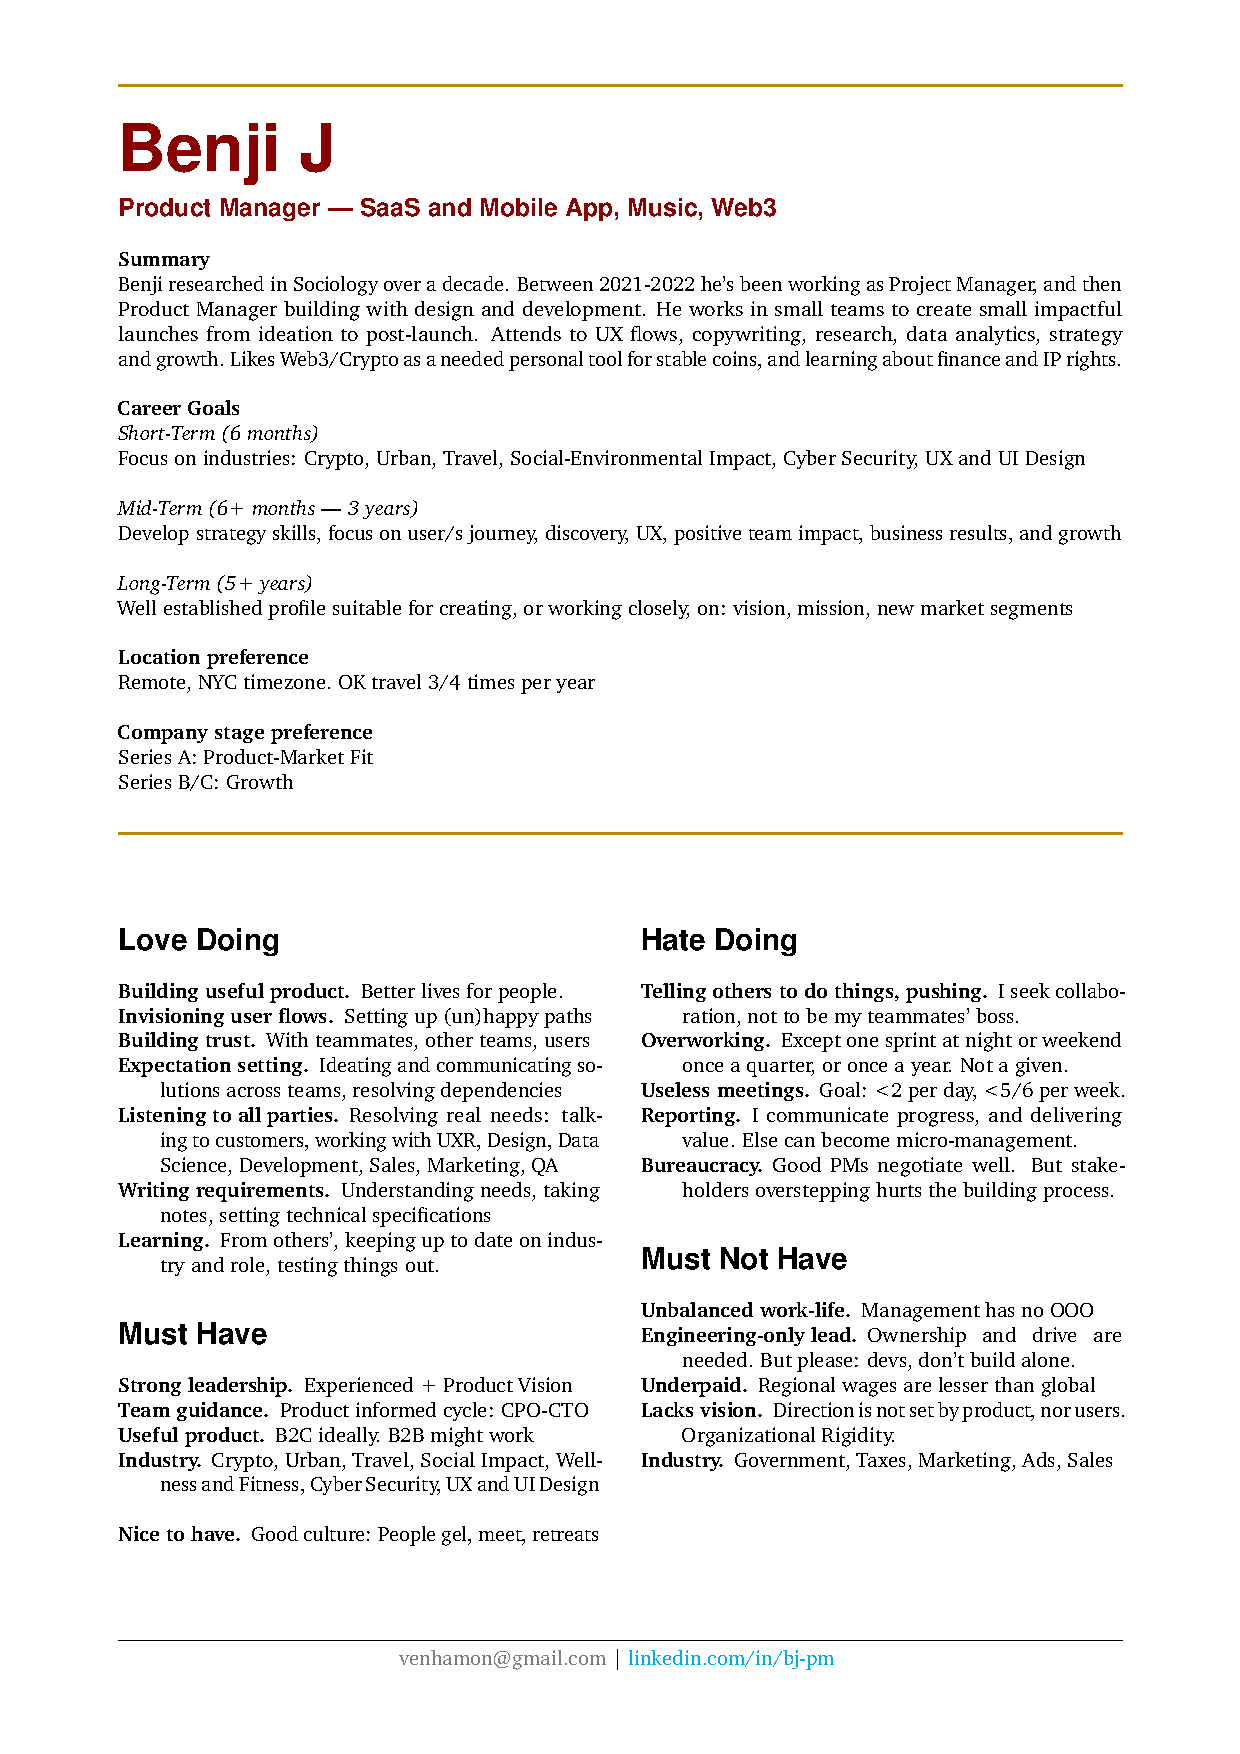
\includepdf[pages={1}]{main.pdf}
%
\maketitle % Print the title
\thispagestyle{firstpage} % IMPORTANT FOOTER
% \thispagestyle{headings}
% \thispagestyle{empty}
% \thispagestyle{plain}
% Apply the page style for the first page (no headers and footers)
% \vfill\eject
% -------------------------------------------------------------
% SUMMARY % ABSTRACT % --------------------------------------------------------------
%
% \vfill\eject
%
%

\section*{Love Doing}

\begin{description}
\item[Building useful product.] Better lives for people. % Good!
% % % % % % % % % % % % % % % % % % % % % % %
\item[Customer Experience.]
Understanding users' journey.
% \item[Getting in customers' shoes.]
% Understanding pain points.
% Solving them, hopefully!
% % % % % % % % % % % % % % % % % % % % % % %
\item[Envisioning user flows.] Setting up (un)happy paths
% % % % % % % % % % % % % % % % % % % % % % %
% \item[Building trust.] With teammates, other teams, users
% % % % % % % % % % % % % % % % % % % % % % %
\item[Listening to all parties.] Resolving real needs: %,
% both external to the company as well as internally
talking to customers,
working with UXR,
Design,
Data Science,
Development,
Sales,
Marketing,
QA.
% C-Level
% \item[Writing requirements.] Understanding needs, %requirements,
% taking notes, setting technical specifications
\item[Problem Solving.]%[Expectation setting.]
Ideating and communicating solutions across teams, resolving dependencies
\item[Delivering.] What impacts most, not late.
\item[Learning.]
From others', %experiences and areas, diving into depth of
keeping up to date on industry and role, testing things out.
\item[Frontend and UI.] Backend is OK, I prefer fullstack.
% % % % % % % % % % % % % % % % % % % % % % %
% Creating an impact on people’s lives, for the better. %- ideally working for a mission-driven company.
\end{description}

\section*{Must Have}

\begin{description}
 \item[Strong leadership.] Experienced + Product Vision
%  Or less Experienced but with Drive and a compelling Roadmap
  \item[Team guidance.] Product informed cycle: CPO-CTO
 \item[Useful product.] B2C ideally. B2B2C works
  \item[Industry.]
  Crypto,
  Urban,
  Travel,
  Social Impact,
  Wellness and Fitness,
  Cyber Security,
  UX and UI Design \\
  \item[Nice to have.]
 Culture: People work well, %relaxed,
 and thrive.
%  gel, meet, retreats %  Great Place to Work is amazing
%   Creative,
%   Entertainment,
%   Health,
\end{description}


% \subsection*{Nice To Have}
% \begin{description}
%  \item lalala
% %  \item lalala
% %  \item lalala
% %  \item lalala
% \end{description}


% \end{document}







% This sentence requires citation \citep{Reference1}. This sentence requires multiple citations to imply that it is better supported \citep{Reference2,Reference3}. Finally, when conducting an appeal to authority, it can be useful to cite a reference in-text, much like \cite{Reference1} do quite a bit. Oh, and make sure to check out the bear in Figure \ref{bear}.

% \onecolumn

% \vfill\eject

% \end{twocolumn}
%
% \begin{twocolumn}

\vfill\eject
% \section*{Hate Doing}

\begin{description}
 \item[Telling others to do things, pushing.]
I don't want to work in a place where goals are not aligned between teams. %which makes it hard to collaborate.
I want to work in a place where peers are motivated and onboarded with
%the goals and
strategy.
I need improvement: a PM role can entail
mentoring and coaching others. %to achieve their goals too.
 %  I seek collaboration, not to be my teammates' boss.
 \item[Overworking.] Except one sprint at night or weekend once a quarter, or once a year.
 Not a given.
 \item[Useless meetings.] Goal: <2 per day,  <5/6 per week. %  No unlimited meeting invites please.
 \item[Reporting.]
%  Stakeholders need to
 I communicate progress, %with focus on
 and delivering value. %, %not presentation.
 Else can become micro-management.
  \item[Bureaucracy.] Good PMs negotiate well.
  % good at handling several stakeholders %can have good outcomes or bad ones % depends on many factors, including company direction:
  But stakeholders overstepping hurts the building process.
% % % % % % % % % % % %
%  I dislike delaying results and delivery:
%  It's OK to chill
%  but  make the product grow, deliver value, on time;
%  for users, team, business.
\end{description}

% \smallskip

%   \vspace*{-20pt}

% \section*{Must Not Have}

\begin{description}
  \item[Unbalanced work-life.] Management has no OOO
  \item[Engineering-only lead.]
  Ownership and drive are needed.
  But please: %building decided by
  devs, don't build alone.
%   only may not lead to good product.
%   with product decisions, not going over the side.
 \item[Underpaid.] Regional wages are lesser than global
 \item[Lacks vision.] Direction is not set by product, nor users. Organizational Rigidity.
  \item[Industry.] Insurance, Government, Taxes, Ads, Sales % Marketing
%  \item[Good Culture.] People actually gel, meet, retreats %  Great Place to Work is amazing
%  \item[Useful Product.] B2C ideally. B2B might work
%   \item[Industry.]
%   Crypto,
%   Urban,
%   Travel,
%   Social Impact
%   Creative,
%   Entertainment,
%   Health,
\end{description}


% This sentence requires citation \citep{Reference1}. This sentence requires multiple citations to imply that it is better supported \citep{Reference2,Reference3}. Finally, when conducting an appeal to authority, it can be useful to cite a reference in-text, much like \cite{Reference1} do quite a bit. Oh, and make sure to check out the bear in Figure \ref{bear}.

% \end{document}


% \section*{Personality}
%
% \subsection*{Myers Briggs}
% \begin{description}
%
% %  \item[INTJ: Architect.] Architects are imaginative and strategic thinkers, with a plan for everything.
%  \item[INTJ: Architect] %Architects are
%  \item[] Imaginative + Strategy / Planning
% %  thinkers, with a plan for everything.
% \end{description}
%
%
%  \subsection*{Enneagram}
%  \begin{description}
%
%  \item[Type 5 / Wing 4 -- The Iconoclast] %\newline
%  \item[] creativeness + sensitivity
% %  is a subtype that results from the encounter of types 5 and 4, which means that the sensitivity of the 4s is added to the natural creativeness of 5s.
%  \end{description}

%  -%Architects are imaginative and strategic thinkers, with a plan for everything.


% \end{document}

% \clearpage
\vspace*{-1.1cm}
\noindent\fbox{%
    \parbox{0.495 \textwidth \fboxsep \fboxsep
    }{% the quick brown fox jumps right over the lazy dog.
%     }%
% }

% \fbox{%
% \begin{minipage}{25em}
% lalala
% \end{minipage}
% }
%
\section*{%Extended
Summary}
\textbf{Candidate-Market Fit [CMF]} \\ %\textit{%
% % 2.
\textit{%
Seeking a \textbf{%
% Senior
Product Manager} role
at an early stage \textbf{%Crypto
startup}, % working closely
with focus on
design and user experience (UX),
on industries like
% FinTech,
FoodTech,
social impact,
and media.
% industries.
%
% Seeking a remote \textbf{Product Manager} role at an early stage (Series C, or younger) B2C company focused on \textbf{Crypto} in the entertainment or media industry.
}
% % 1.
% % Seeking a remote \textbf{Product Manager} role with attention to UX at an early stage (Series C, Pre-IPO/ICO) \textbf{Crypto} B2C company with emphasis on social impact, real-life assets, music and media industries.
% \textit{
% \#crypto
% \#IP-rights
% \#real-world-assets
% \#music
% \#streaming
% \#growth
% \#transformation
% \#AI
% \#UX
% \#B2C
% \#B2B
% }
% \#B2B2C
% \#design
% \\
% \#NFTs
% \#B2B
% % Seeking a Product Manager remote role with attention to UX at a Series-A to C SaaS-based tech company in Crypto, ideally with social impact, B2C or B2B2C.
% % Ideal: based in Argentina or Latin America, in Spanish or Portuguese.
% % \\
% % Location preference: Remote, NYC timezone. OK travel 3/4 times per year
% % \\ \\
% % \textit{%
% % Seeking a Product Manager remote role
% % with attention to UX
% % at a Series-A/C SaaS-based tech company in Crypto,
% % ideally with social impact, B2C. \\
% % Ideal:
% % Argentina/Latin America,
% % Spanish/Portuguese.
% % }
% % \\ \\
% My background is in sociology and systems analysis: now inclining towards data analytics to inform product decisions. \\ \\
% I enjoy user feedback roles, discovery and testing.
% I'm OK with public presentations: I like sharing ideas and asking for collaboration both with internal teams, as well as with
% users,
% audience and
% other companies.
% \\
% Open to growth roles focused on customer experience.
% Prefer a role that includes other Product Manager, or near: above or below.
% Interested in joining a start-up in an in-demand industry. % % % % % % % % %
% If given a choice, my
\subsection*{%
% Preferred
% areas:
Best Industries:
% Crypto/Blockchain/Web3
% crypto, or not
}
\begin{description}
%  \item[Crypto]
\item[Social:]
FoodTech,
Ed Tech,
% FinTech,
Fundraising,
Travel % Urban
\item[Entertainment:] Music,
Gaming,
Publishing
% \item[Productivity:]
\item[Product:]
Transformation,
Task Management Systems
% UX/UI Design
\item[Wellbeing:] Meditation, Sleep, Social Impact, Health % Fitness,
% \item[B2B/B2B2C:]
% Cyber Security,
\end{description}
\\ \\
\subsection*{Company stage preference}     \\
Series A:
Product-Market Fit
% Series C: Growth \\
% Series B/C: Growth
% I am open to other opportunities as I do not have direct industry experience in these fields.
% My background is in sociology and systems analysis. I enjoy user feedback roles, discovery and beta testing.


% This sentence requires citation \citep{Reference1}. This sentence requires multiple citations to imply that it is better supported \citep{Reference2,Reference3}. Finally, when conducting an appeal to authority, it can be useful to cite a reference in-text, much like \cite{Reference1} do quite a bit. Oh, and make sure to check out the bear in Figure \ref{bear}.

% \onecolumn
% \end{minipage}
% }

% \noindent\fbox{%
%     \parbox{0.47 \textwidth \fboxsep \fboxsep}{%
%     hello
\section*{Must Have}

\begin{description}
 \item[Strong leadership.] Experienced + Product Vision
%  Or less Experienced but with Drive and a compelling Roadmap
  \item[Team guidance.] Product informed cycle: CPO-CTO
 \item[Useful product.] B2C ideally. B2B2C works
  \item[Industry.]
  Crypto,
  Urban,
  Travel,
  Social Impact,
  Wellness and Fitness,
  Cyber Security,
  UX and UI Design \\
  \item[Nice to have.]
 Culture: People work well, %relaxed,
 and thrive.
%  gel, meet, retreats %  Great Place to Work is amazing
%   Creative,
%   Entertainment,
%   Health,
\end{description}


% \subsection*{Nice To Have}
% \begin{description}
%  \item lalala
% %  \item lalala
% %  \item lalala
% %  \item lalala
% \end{description}


% \end{document}







% This sentence requires citation \citep{Reference1}. This sentence requires multiple citations to imply that it is better supported \citep{Reference2,Reference3}. Finally, when conducting an appeal to authority, it can be useful to cite a reference in-text, much like \cite{Reference1} do quite a bit. Oh, and make sure to check out the bear in Figure \ref{bear}.

% \onecolumn

% \vfill\eject

% \end{twocolumn}
%
% \begin{twocolumn}


    }%
}

\vfill\eject
\section*{Strengths \& Weaknesses}

My Strengths are based on my Gallup Strengths:
\begin{description}
 \item [Believer]
 \item [Philomath]
 \item [Coach]
 \item [Self-Believer]
 \item [Strategist]
\end{description}

% \noindent
% My areas to improve come from Personality overall.

\subsection*{Strengths}

\begin{description}
 \item[Belief] in: people's capabilities and that they can bring a lot to the table, from both a work and personal view.
 self, others, team, company.
 My view %of the company and team
 makes me %super
 high drive, and persistent.
\item[Curious.] I love learning, but my fuel is in placing questions forward and not staying stagnant with a simple eternal answer. Iteration and nuance are key.
\item[Supportive.] I push causes to happen, and I believe we can all give something out to the world. wagmi: we're all gonna make it.
\item[Ownership.] I believe to have both confidence and certainty to move forward, and I strive for other people to gain them as well.
\item[Strategist.] Always aiming for the big picture: am I going to be happy about this work in 20 to 50/200 years? I hope so. Let's plan steps and execute!
 \end{description}

\subsection*{Weaknesses}

\noindent
My areas to improve come from Personality overall:
INTJ
+
Type 5 / Wing 4

\begin{description}
 \item[Contrarian:] sometimes wrongly, :P
 \item[] \> \> \>
%  \hrule
%  $ $ $ $
 I believe in people's intent and their heart-felt beliefs and actions. At the same time,
 I can disagree with their ideas and perspectives,
 and it's a challenge to communicate both angles.
%  at the same time
 \item[Interruptor:] a fine art that ought never be learned :P \\
 I get excited about a conversation and want to contribute. Video calls do help with this:
 because you have to unmute, and really
 check if the other person is OK and wrapped their idea.
%  pay attention to pauses in conversation before speaking.
 \item[Overly Imaginative:] going off rail to derivatives can be unproductive for working on immediate goals. Let's better plan one step at a time %so we can
 to stay in sync
 \item[Data insufficient:] I'm biased to teamwork and intuition. It's OK to build quickly and iterate, but %it would  be
 it's best to plan strategies with hard-data. % based decisions.
 It's one of my next steps, but not there yet.
%  \item[Unexperienced Professional Background:] no well-known, big-name company on my resume as an employer. Primary experience in unstructured companies, mostly regional, in LatinAmerica, and in a promising Music Startup (with HQ in US and Europe) but that hasn't yet gained traction.
%  \item[]
\item[Stakeholder Influence.] Even though I feel in general to have good relationships across teams, I may need to review what my leverage is, and how much I can or should influence across company.
 \end{description}

\section*{Personality}

% \subsection*{Gallup Strengths (*)}
% \begin{description}
%  \item [Believer]
%  \item [Philomath]
%  \item [Coach]
%  \item [Self-Believer]
%  \item [Strategist]
% \end{description}



\subsection*{Myers Briggs}
\begin{description}

%  \item[INTJ: Architect.] Architects are imaginative and strategic thinkers, with a plan for everything.
 \item[INTJ: Architect]
 Introversion (I),
 Intuition (N), \\
 Thinking (T),
 Judgment (J)
 \item[] Imaginative + Strategy / Planning
%  thinkers, with a plan for everything.
\end{description}


 \subsection*{Enneagram}
 \begin{description}

  \item[Type 5: The Investigator] %\newline
 \item[/ Wing 4: The Iconoclast] %\newline
 \item[] creativeness + sensitivity
%  is a subtype that results from the encounter of types 5 and 4, which means that the sensitivity of the 4s is added to the natural creativeness of 5s.
 \end{description}

%  -%Architects are imaginative and strategic thinkers, with a plan for everything.


% \noindent\fbox{%
%     \parbox{0.49 \textwidth \fboxsep \fboxsep}{%

\subsection*{Dream Idea}

\begin{description}
 \item[Earthworms everywhere:] %sharing, %in a chain,
 like \href{https://www.imdb.com/title/tt0223897/}{Pay It Forward (2000)}.
%  \item \> \> \>
 I've already
%  have the know-how to
 given away vermicomposting materials for recycling
 over a decade. %  to one person at a time, and have been doing so for almost a decade.
But how do you create a chain reaction? Do others want to spread the word, the earthworms, and recycling in every home around the globe?
\end{description} \\ \\
%     }%
% }


\vfill\eject

\end{document}


\clearpage

% \begin{center}\rule{0.5\linewidth}{0.5pt}\end{center}

\section*{Benji's career plan}


\hypertarget{year-1-strengthening-core-skills-and-network}{%
\subsubsection*{\texorpdfstring{\textbf{Year 1: Strengthening Core Skills}}{Year 1: Strengthening Core Skills and Network}}\label{year-1-strengthening-core-skills-and-network}}

\begin{itemize}
\tightlist
\item
  \textbf{Goal}: Deepen expertise in blockchain and product management
  within the social impact space.

  \begin{itemize}
  \tightlist
  \item
    \textbf{Q1/Q2}: Take certifications @scrum.org:
    Scrum Master,
    Product Owner
%     (e.g., Certified Blockchain
%     Professional or a PM certification).
  \item
    \textbf{Q2/Q3}: Attend and actively participate in at least one major
    industry conference or event related to crypto or social impact,
    such as Consensus or TechCrunch Disrupt.
  \item
    \textbf{Q3/Q4}: Continue a personal project from 2023 or contribute to an
    open-source project in the social impact space, focusing on using
    blockchain for good.
  \item
    \textbf{Q4}: Build and nurture relationships with key players in the
    social impact and blockchain communities through networking events,
    LinkedIn, and other platforms.
  \end{itemize}
\end{itemize}

\hypertarget{year-2-expanding-influence-and-impact}{%
\subsubsection*{\texorpdfstring{\textbf{Year 2: Expanding Influence and
Impact}}{Year 2: Expanding Influence and Impact}}\label{year-2-expanding-influence-and-impact}}

\begin{itemize}
\tightlist
\item
  \textbf{Goal}: Increase visibility and thought leadership within the
  industry.

  \begin{itemize}
  \tightlist
%   \item
%     \textbf{Q1}: Write and publish 2-3 articles on Medium or LinkedIn about blockchain's role in social impact, sharing insights from your projects and experience.
  \item
    \textbf{Q1/Q2}: Mentor a junior product manager or blockchain
    enthusiast, offering guidance based on your experience in crypto and
    pre-seed incubation.
  \item
    \textbf{Q2/Q3}: Lead or co-lead a workshop or webinar on blockchain and
    social impact at a conference or community event.
  \item
    \textbf{Q4}: Explore opportunities for collaboration with NGOs or
    social enterprises, potentially advising or consulting on blockchain
    solutions.
  \end{itemize}
\end{itemize}

\hypertarget{year-3-transitioning-to-leadership-roles}{%
\subsubsection*{\texorpdfstring{\textbf{Year 3: Transitioning to
Leadership
Roles}}{Year 3: Transitioning to Leadership Roles}}\label{year-3-transitioning-to-leadership-roles}}

\begin{itemize}
\tightlist
\item
  \textbf{Goal}: Move into a senior product management role or begin
  exploring entrepreneurial opportunities.

  \begin{itemize}
  \tightlist
%   \item
%     \textbf{Q1}: Apply for senior product management roles with a focus
%     on blockchain and social impact within innovative companies or
%     startups.
  \item \textbf{Q1}: Spearhead a project that leverages blockchain for social good, such as developing a new product or improving an existing one.
  \item \textbf{Q2/Q3}: Consider starting your own venture or joining an early-stage startup as a co-founder or key team member, focusing on blockchain solutions for social impact.
  \item
    \textbf{Q4}: Continue to build your public profile through speaking
    engagements, panel discussions, or being featured in industry
    podcasts.
  \end{itemize}
\end{itemize}

\bigskip

\hypertarget{year-4-5-establishing-authority-and-broadening-horizons}{%
\subsubsection*{\texorpdfstring{\textbf{Years 5-10: Establishing Authority
and Broadening
Horizons}}{Years 5-10: Establishing Authority and Broadening Horizons}}\label{year-4-5-establishing-authority-and-broadening-horizons}}

\begin{itemize}
\tightlist
\item
  \textbf{Goal}: Solidify your position as a thought leader and
  potentially transition to a founder or executive role.

  \begin{itemize}
  \tightlist
  \item
    \textbf{Year 5}:

    \begin{itemize}
    \tightlist
    \item
      Scale your impact by leading a major product or initiative that
      achieves significant social outcomes using blockchain.
    \item
      If entrepreneurial, secure funding for your startup and lead it
      through a successful launch.
    \end{itemize}
  \item
    \textbf{Year 10}:

    \begin{itemize}
    \tightlist
    \item
      Become a recognized authority in the intersection of blockchain,
      product management, and social impact, with regular invitations to
      speak at top-tier conferences.
    \item
      Consider publishing a book or extensive guide on blockchain for
      social good.
    \item
      If your startup has gained traction, consider expansion or
      exploring new markets.
    \end{itemize}
  \end{itemize}
\end{itemize}

% This plan is designed to build on Benji's existing strengths while
% expanding their influence and leadership in the industry. It also allows
% for flexibility in either deepening expertise within organizations or
% pursuing entrepreneurial ventures.

% \begin{center}\rule{0.5\linewidth}{0.5pt}\end{center}


% \end{twocolumn}
%
% \begin{twocolumn}


% \section*{Not Good}
%
%
% Lorem ipsum dolor sit amet, consectetur adipiscing elit. Fusce maximus nisi ligula. Morbi laoreet ex ligula, vitae lobortis purus mattis vel. Vestibulum ante ipsum primis in faucibus orci luctus et ultrices posuere cubilia Curae; Donec ac metus ut turpis mollis placerat et nec enim. Duis tristique nibh maximus faucibus facilisis. Praesent in consequat leo. Maecenas condimentum ex rhoncus, elementum diam vel, malesuada ante. Fusce pulvinar, mauris pretium placerat venenatis, lectus ex tempus lacus, id suscipit libero lorem eu augue. Interdum et malesuada fames ac ante ipsum primis in faucibus.
%
% \vfill\eject
%
% \section*{Hate}
%
% \begin{description}
%  \item[Underpaid.] Regional wages are lesser than global
%   \item[Unbalanced work-life.] Management has no OOO
%     \item[Engineering Lead.] Building decided by devs only
%  \item[Lacks Vision.] Direction is not set by product, nor users
%   \item[Industry.] Government, Taxes, Marketing, Ads, Sales
% %  \item[Good Culture.] People actually gel, meet, retreats %  Great Place to Work is amazing
% %  \item[Useful Product.] B2C ideally. B2B might work
% %   \item[Industry.]
% %   Crypto,
% %   Urban,
% %   Travel,
% %   Social Impact
% %   Creative,
% %   Entertainment,
% %   Health,
% \end{description}
%
% \smallskip
%
% \section*{Must Not Have}
%
% \begin{description}
%  \item[Underpaid.] Regional wages are lesser than global
%   \item[Unbalanced work-life.] Management has no OOO
%     \item[Engineering Lead.] Building decided by devs only
%  \item[Lacks Vision.] Direction is not set by product, nor users
%   \item[Industry.] Government, Taxes, Marketing, Ads, Sales
% %  \item[Good Culture.] People actually gel, meet, retreats %  Great Place to Work is amazing
% %  \item[Useful Product.] B2C ideally. B2B might work
% %   \item[Industry.]
% %   Crypto,
% %   Urban,
% %   Travel,
% %   Social Impact
% %   Creative,
% %   Entertainment,
% %   Health,
% \end{description}



% \end{document}

%%%%%%%%%%%%%%%%%%%%%%%%%%%%%%%%%%%%%%%%%
% Wenneker Article
% LaTeX Template
% Version 2.0 (28/2/17)
%
% This template was downloaded from:
% http://www.LaTeXTemplates.com
%
% Authors:
% Vel (vel@LaTeXTemplates.com)
% Frits Wenneker
%
% License:
% CC BY-NC-SA 3.0 (http://creativecommons.org/licenses/by-nc-sa/3.0/)
%
%%%%%%%%%%%%%%%%%%%%%%%%%%%%%%%%%%%%%%%%%

%----------------------------------------------------------------------------------------
%	PACKAGES AND OTHER DOCUMENT CONFIGURATIONS
%----------------------------------------------------------------------------------------


%----------------------------------------------------------------------------------------
%	ABSTRACT
%----------------------------------------------------------------------------------------

% \lettrineabstract{Lorem ipsum dolor sit amet, consectetur adipiscing elit. Fusce maximus nisi ligula. Morbi laoreet ex ligula, vitae lobortis purus mattis vel. Vestibulum ante ipsum primis in faucibus orci luctus et ultrices posuere cubilia Curae; Donec ac metus ut turpis mollis placerat et nec enim. Duis tristique nibh maximus faucibus facilisis. Praesent in consequat leo. Maecenas condimentum ex rhoncus, elementum diam vel, malesuada ante.}

%----------------------------------------------------------------------------------------
%	ARTICLE CONTENTS
%----------------------------------------------------------------------------------------

% \section*{Good}
%
% \begin{description}
%  \item[Strong Leadership.] Experienced + Product Vision
% %  Or less Experienced but with Drive and a compelling Roadmap
%  \item[Good Culture.] People actually gel, meet, retreats %  Great Place to Work is amazing
%  \item[Useful Product.] B2C ideally. B2B might work
%   \item[Industry.] Entertainment, Creative, Travel, Health
% \end{description}

% This sentence requires citation \citep{Reference1}. This sentence requires multiple citations to imply that it is better supported \citep{Reference2,Reference3}. Finally, when conducting an appeal to authority, it can be useful to cite a reference in-text, much like \cite{Reference1} do quite a bit. Oh, and make sure to check out the bear in Figure \ref{bear}.


% % % % % % % % % % % % % % % % %

% 10pt font size (11 and 12 also possible), A4 paper (letterpaper for US letter) and two column layout (remove for one column)
% \usepackage[1]{pagesel}
% https://tex.stackexchange.com/questions/96256/compiling-only-a-page-range-or-page-selection


% % % % % % % % % % % % % % % % % % % % % % % % % % % % % % %



% % % 2024-08-01 Lucas Martinez / Coaching, Session 1
% % %
% % % TAREA LinkedIn Revamp
% % % TAREA Hacer Lista de skills
% transferibles
% no transferibles

% %  TAREA entrar a linkedin a buscar laburo remote de product manager

% Muchos trabajos diferentes!
% poco tiempo!
% entra y se va!
% 1/2 anios break-even point
% sacar meses cortos
% de que manera hay una historia!?
%  eliminar laburos cortos
%  acomodar fechas de laburo un mes, estirar, para que no sea tan saltarin
% technical writer, que relacion tiene con lo que quiero lograr > strategic / Product Marketing Manager specialist


% %  cuales son mis skills? que traigo de lo academico
% % sueldo de egresado // 80K
% %  150K muy buen sueldo, medio techo
% % 250K sr manager
% % de ahi para arriba hay pocos roles
% % yo deberia poder 100-150K en EEUU

